\chapter{Background} 
\todo{Meeting notes}
% Software product lines, previous publication (pinpoint what can be improved), SOS rules and operational semantics, and what is modular analysis
% Background should not contain many of my results, but rather retelling what software product lines are, what operational semantics are, existing technologies
% % What is the difficulty of doing analysis on it? Just explaining the structures does not convey why it is worth spending time to solve the problems. Hint at what is coming, that this is something I will tackle in the contribution. 
% Can't be technical in the introduction, the background is where I introduce the terms and definitions and technical details. And the implications of these details.
% Explain what I mean by "modularity", explain why the previous work is not modular. 
% What do I assume, and what do I focus on

\section{Software product lines}
\label{sec:software-product-lines}
\subsection{Feature models}
\label{sub:feature-models}
\begin{figure}
   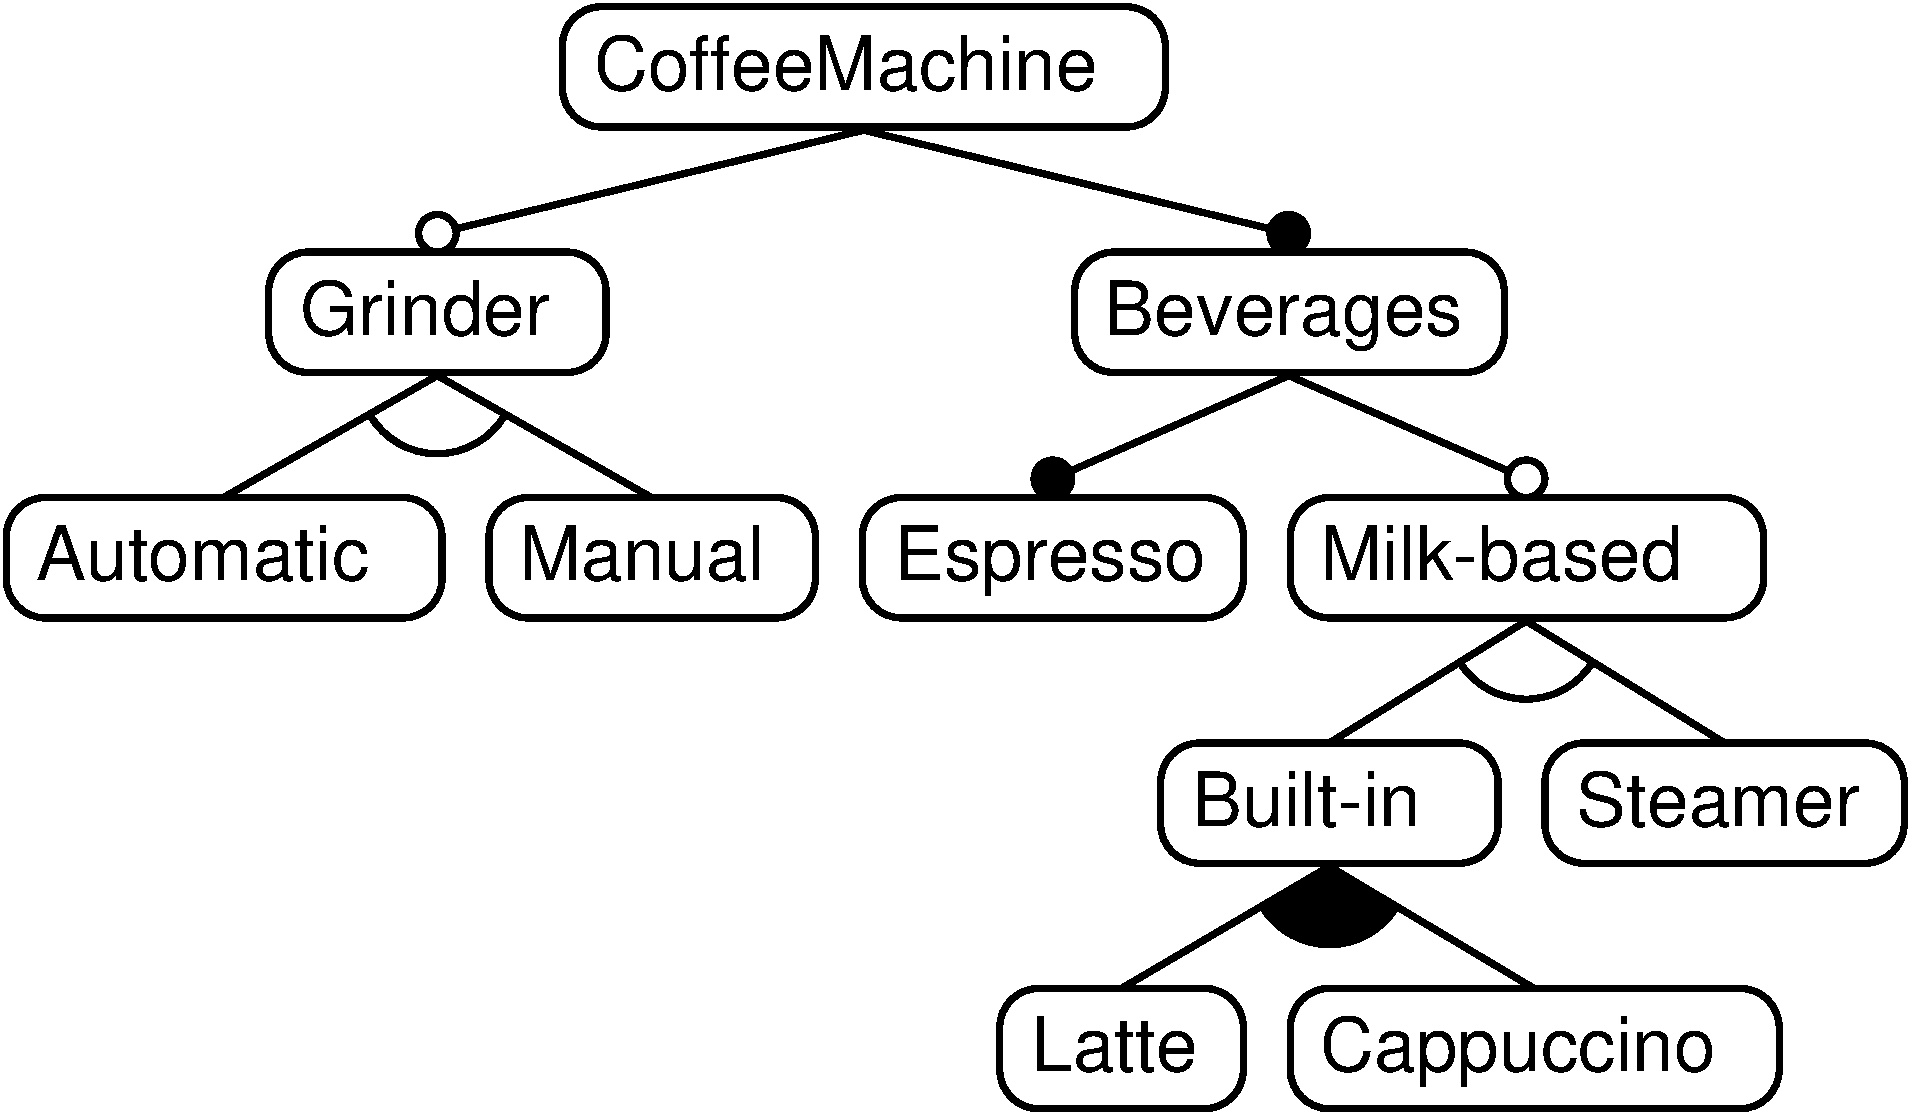
\includegraphics[width=\textwidth]{CoffeeMachine1.pdf}
   \caption[Example feature model for a coffee machine]{Example feature model for a coffee machine \protect\footnotemark}
   \label{ex:fm-coffee1}
\end{figure}

To model the relations between the features (which combinations are allowed, which are common to all variants, etc.), it is common to use a \emph{feature model}. A feature model is a tree-like structure where the nodes are features and groups of features. See figure \vref{ex:fm-coffee1} for an example of a feature model. A feature cannot be selected in a variant unless its parent feature is also selected.

A group gives logical structure to the features, restricting the allowed combinations of the features. For instance, in an \emph{alternative} group, exactly one of the features must be selected in every variant. In the example, the group under Grinder has this type. In a variant, a grinder cannot be both automatic and manual. Moreover, the features have types (\optional{} and \mandatory{}). A \mandatory{} feature must be selected in all variants, whereas an \optional{} feature may be left out. The black dot above Beverages means that this feature is mandatory, so all coffee machines provide beverages. Furthermore, since its subfeature Espresso is also mandatory, all coffee machines have espresso. However, only some coffee machines have milk-based drinks, as shown by the white dot above the Milk-Based feature. If selected, then either built-in drinks such as latte or cappuccino must be included in the variant, or the machine must have a steamer so the user can make milk-based drinks themselves. The group under Built-in is filled-in with black, which means that it is an \emph{or} group. In a variant where Built-in is chosen, one or both of Latte and Cappuccino must also be chosen, but not zero. The groups which are neither \xortype{} nor \ortype{} have the type \andtype{}, which means that zero, one, or more of its subfeatures may be selected in a variant. There are several restrictions to the structure of a feature model. For instance, an \xortype{} or \ortype{} group cannot contain a \mandatory{} feature. The root feature (here CoffeeMachine) must have type \mandatory{}, since naturally it must be selected in all variants.

Feature models often also allow \emph{cross-tree constraints}. These are similar to the parent-child relation in the feature model, but are independent of the tree structure. For instance, one could imagine that the producer would always include an automatic grinder if the Built-In feature is selected, because the built-in feature does not work unless the machine grinds the coffee automatically. This cross-tree constraint could be expressed as "Built-In requires Grinder``. Although cross-tree constraints are commonly used, we disregard them in this thesis. This is due to the fact that the cross-tree constraints add unwanted complexity, and we wish to exploit the tree structure of a feature model.

\subsection{Feature model evolution plans}
\label{sub:feature-model-evolution-plans}
The evolution of an SPL can be planned using a \emph{feature model evolution plan}. Software product lines often grow very large, and it is crucial to plan ahead.


\section{Static analysis}
\label{sec:static-analysis}

Give static analysis \emph{way of thinking} as background, not the exact methods used to analyse programs, but the principles such as may/must analysis etc. Explain how it is communicated (rules), how scope is a factor and discuss soundness in static analysis context (this is the same as the soundness I talk about). 

In static analysis of programs, it is impossible to have both soundness, completeness, and automation. Thus one must prioritize. For some kinds of analysis, it is better with false positives than false negatives, which gives us completeness but we sacrifice soundness. In other cases, it is better to have false negatives than false positives, in which case we sacrifice completeness but gain soundness.

Unlike programs, it is possible to get full overview of a feature model evolution plan. It is always possible to find the correct answer given the question "Does feature A exist at time 5?". An operational representation finds the answer by applying operations to the initial model until time 5 is complete, and checks if feature A exists in the resulting feature model. For intuition on why this must be true, imagine a (correct) program where we know all statements are assignment. This program terminates for a certainty, since there is no branching. The same goes for an operational feature model evolution plan. There are no conditional statements and thus no branching. Since we know that every operational feature model evolution plan ``terminates", we avoid the halting problem which is at the core of all static analysis of programs, which must always over- or under-approximate a solution to be certain that the analysis terminates.

\footnotetext{Created using DarwinSPL: \url{https://gitlab.com/DarwinSPL/DarwinSPL}} %TODO: Move this to the correct page
% Static analysis is semantic-based analysis. Syntax-driven, but semantic-based, but also of the meaning. If we have x := 5, then it means that 5 is the value which you put into x
% Say that I'm doing semantic-based analysis in the thesis, _analysis_, not just semantics.Can I add it or not? How much of the scope is affected? Emphasize modularity; analysis is modular. Focus on the analytical parts of the work, combined with the semantics of a feature model
% Don't call the rules SOS rules, but "Rules for semantics-based analysis". Stop downplaying
% Give the structure of the rules in the background. Static analysis has an environment and an effect. I'm making a calculus
% Analysis is formalized through a set of rules, which often have this kind of structure... which also looks very much like SOS rules.
% Emphasize that I've made an implementation as well as the theory.
\subsection{Analysis context (rules)}
\label{sub:analysis-context}
% How a rule can represent an environment
\subsection{Soundness}
